\begin{figure*}[t]
    \centering
    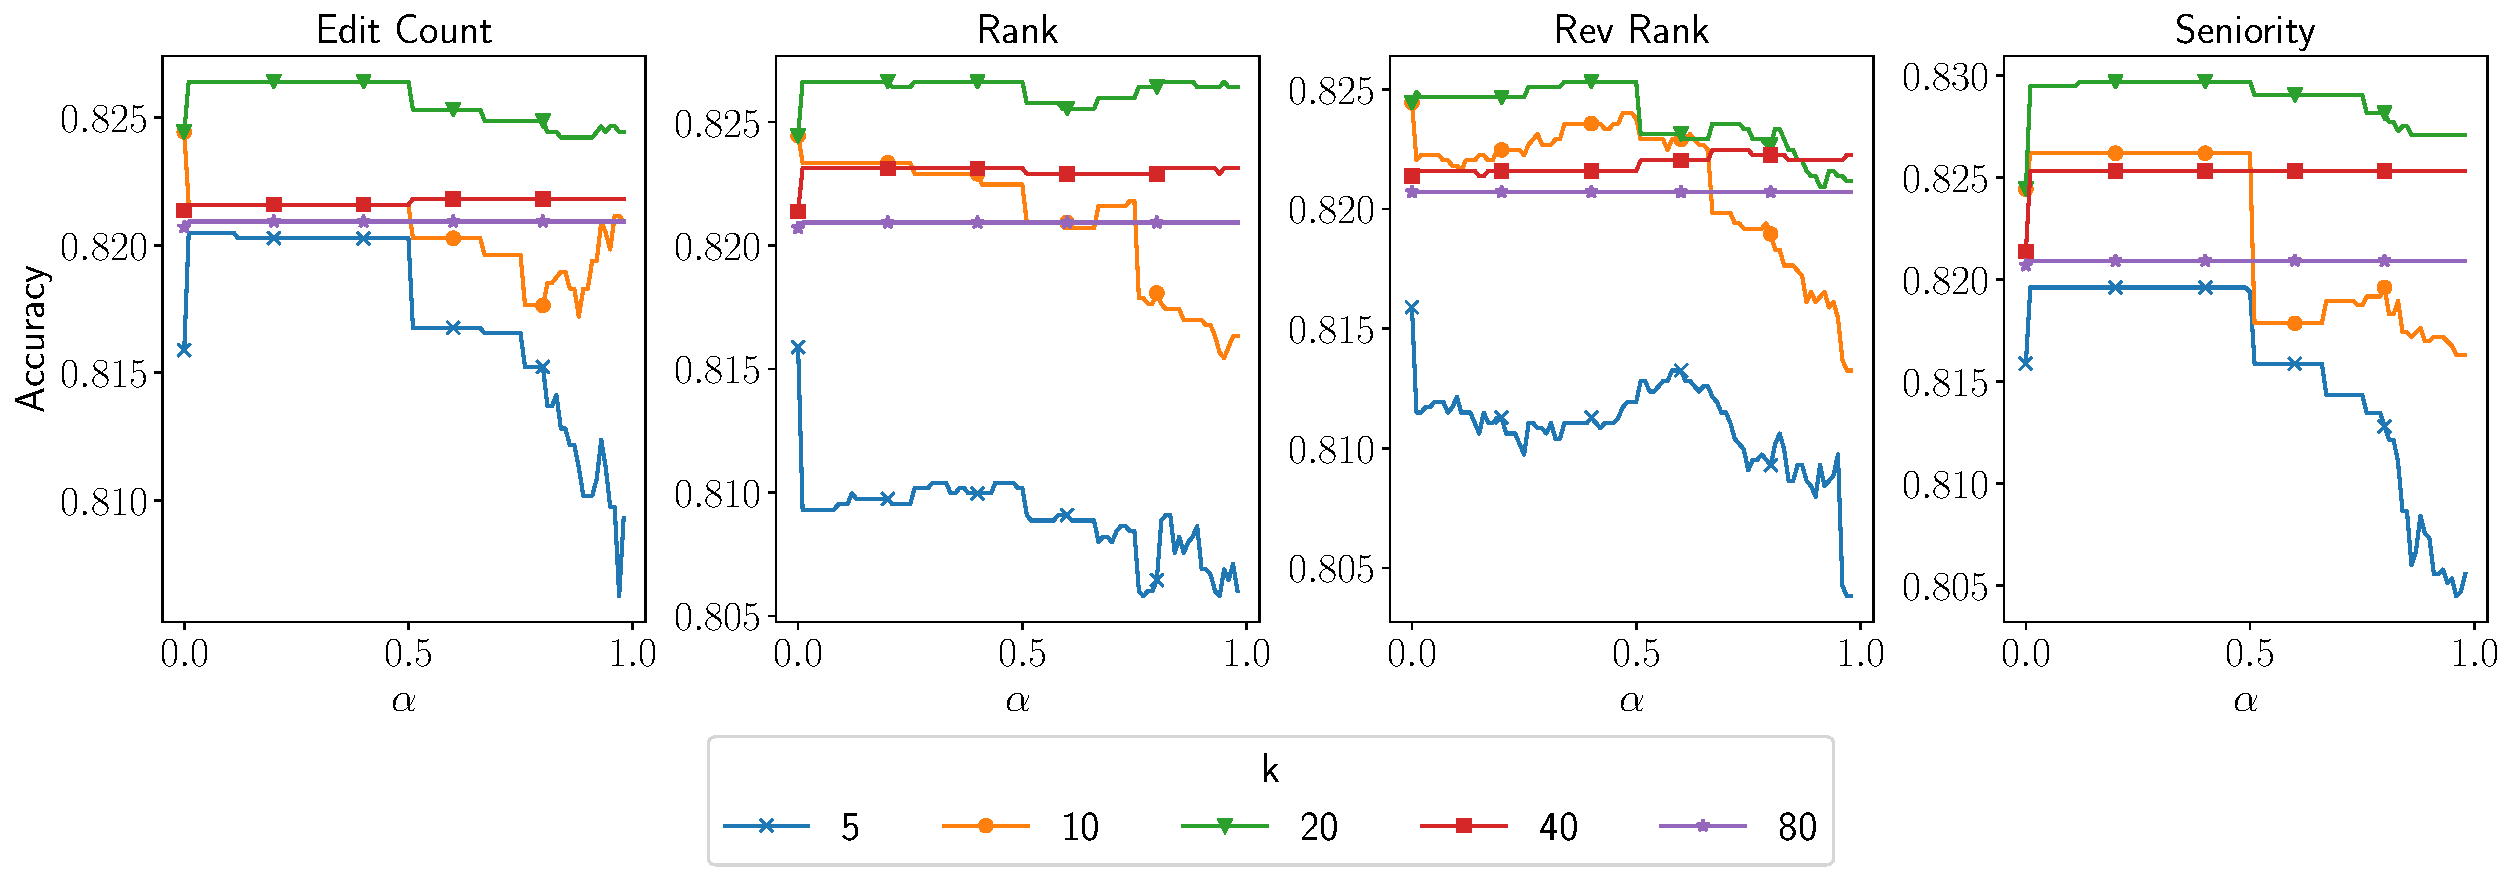
\includegraphics[width=\linewidth]{images/alpha_local.pdf}
    \caption{Effect of $\alpha$ for the \localv model with different delegation rules and values of $k$}
    \label{fig:local-alpha}
\end{figure*}
\begin{figure*}[t]
    \centering
    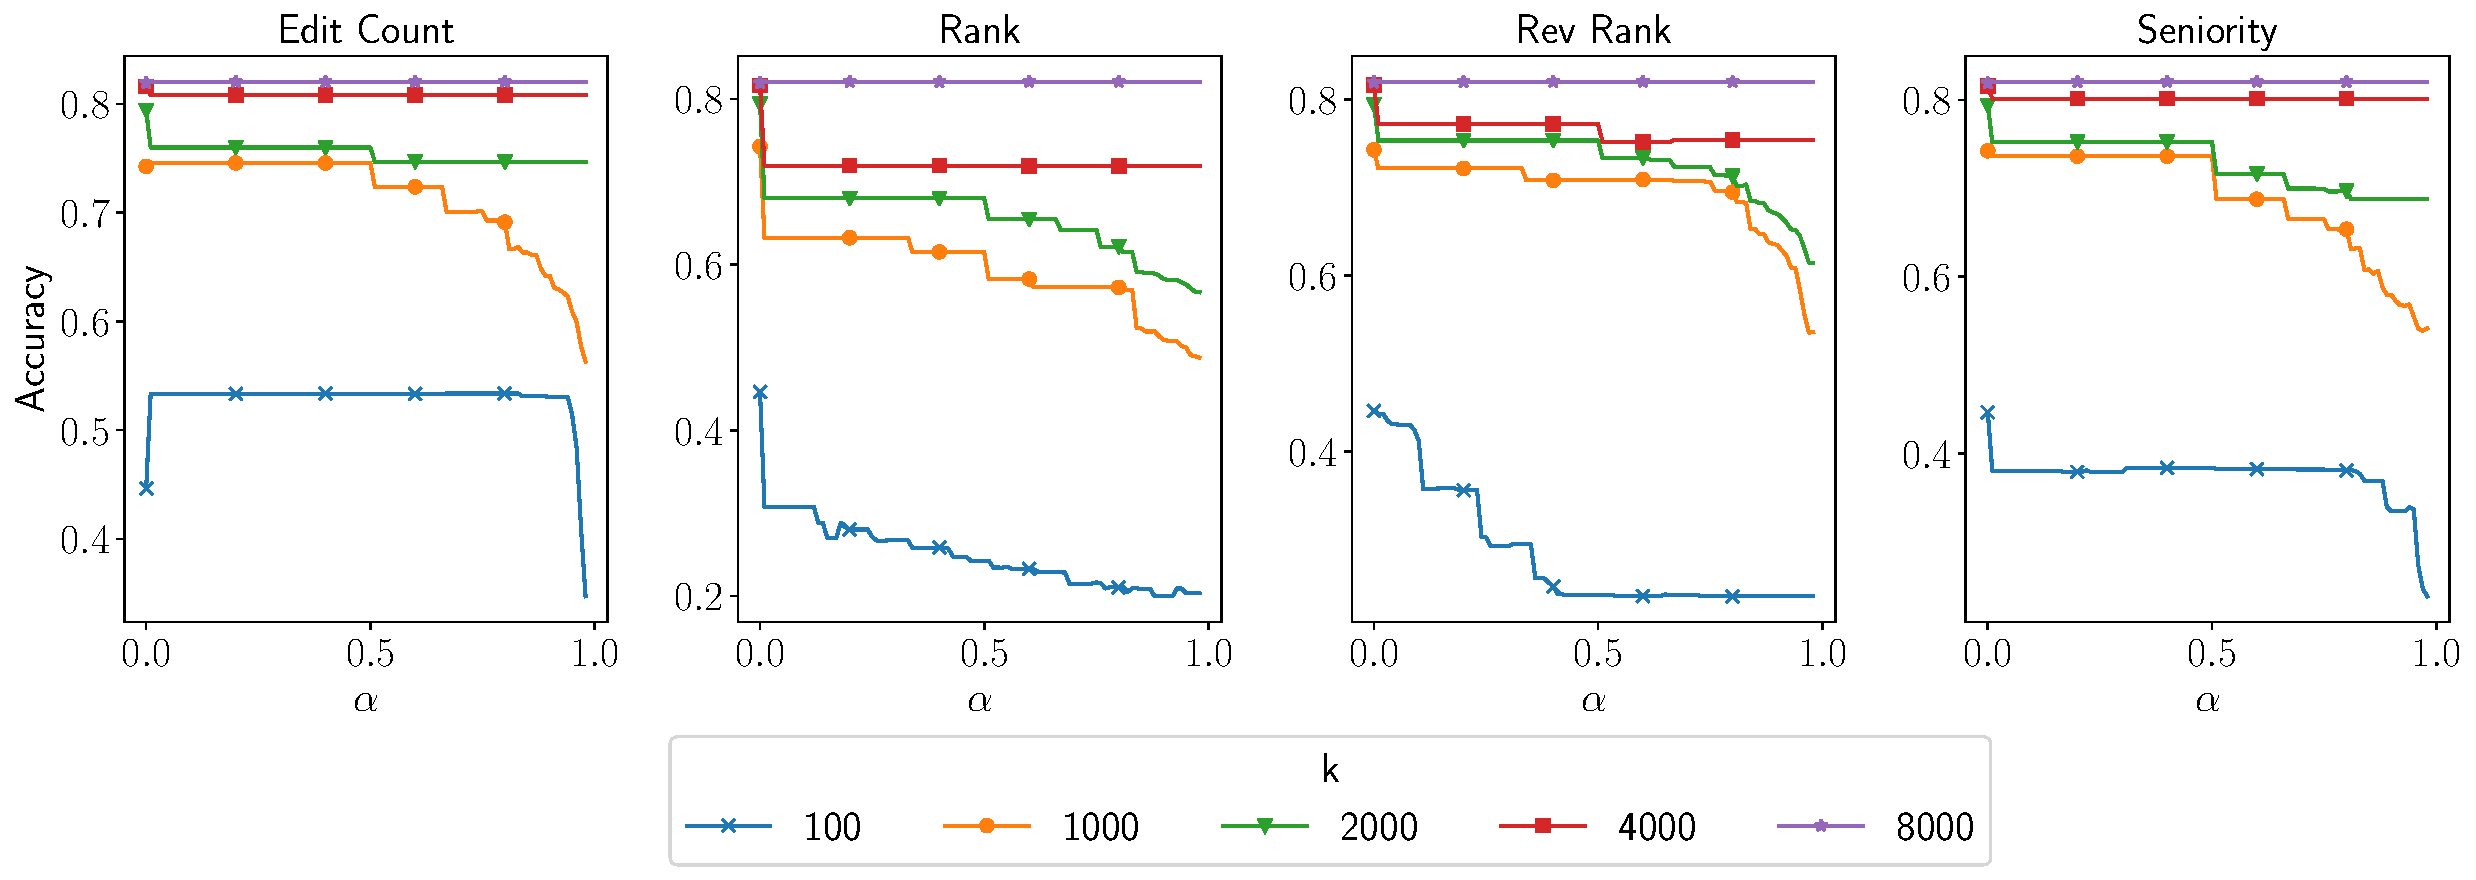
\includegraphics[width=\linewidth]{images/alpha_global.pdf}
    \caption{Effect of $\alpha$ for the \globalv model with different delegation rules and values of $k$}
    \label{fig:global-alpha}
\end{figure*}

\section{Results and Discussion}

\label{sec:results}
In this section, we present the results of the viscous democracy model and analyse the effects of the various parameters on the accuracy of the model.

The main metric we will be using to compare the quality of the Viscous Model is \textbf{accuracy}. The baseline that will be used to measure the model against is a simple tally of all the votes in an RfA election. This compares the most directly with our models as we increase the value of $k$. The baseline model of just tallying the votes gives an accuracy of $\mathbf{82\%}$. 

There are many parameters that have an effect on the predictive accuracy of the model. This means that the effective size of search space is quite large especially as parameters like $\alpha$ have a continuous domain. To narrow the search space as well as to gain a better understanding of the effects each parameter has on the model we fix all others and take a closer look in the following subsections. Finally we discuss the results of the grid search over the pruned parameter space to find the best performing model.

\begin{figure*}[t]
    \centering
    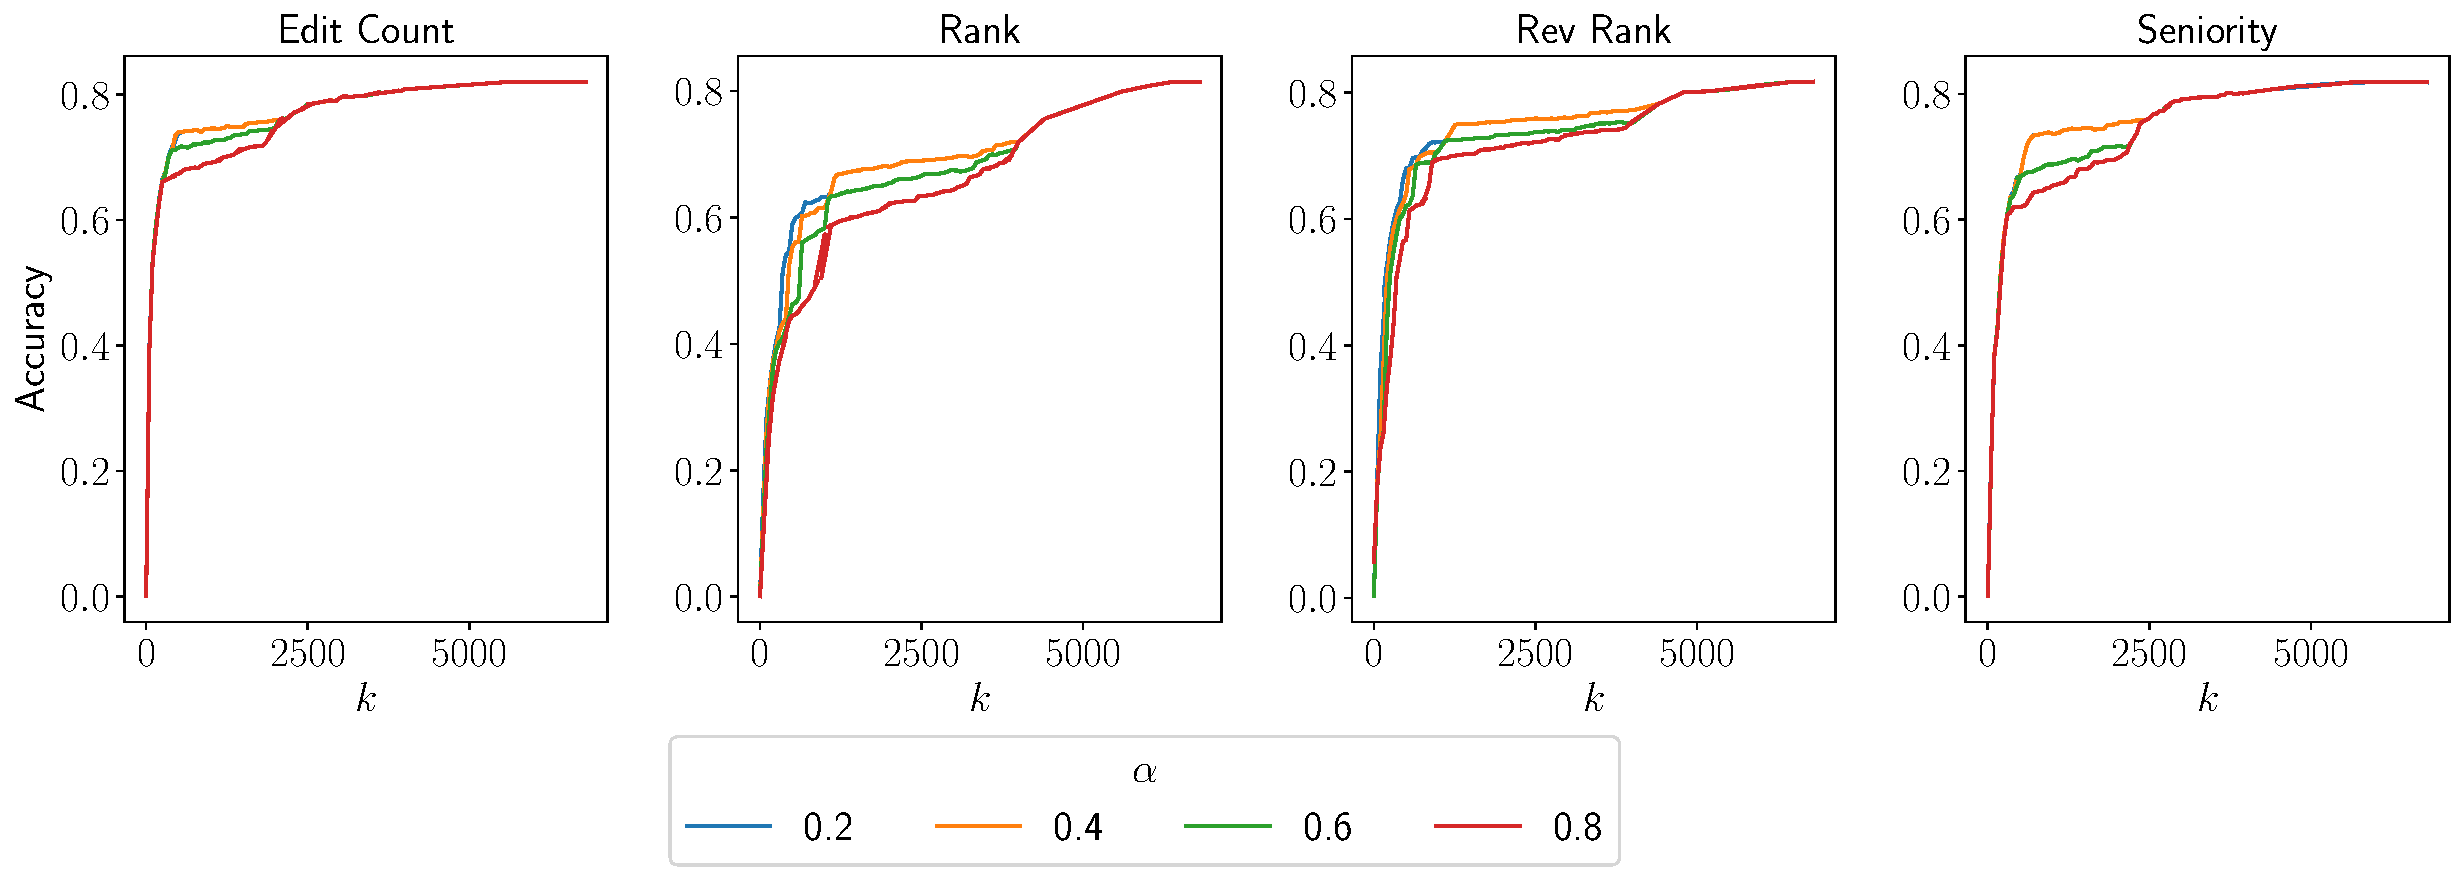
\includegraphics[width=\linewidth]{images/k_global.pdf}
    \caption{Effect of $k$ for the \globalv model with different delegation rules and values of $\alpha$}
    \label{fig:global-k}
\end{figure*}
\begin{figure*}[t]
    \centering
    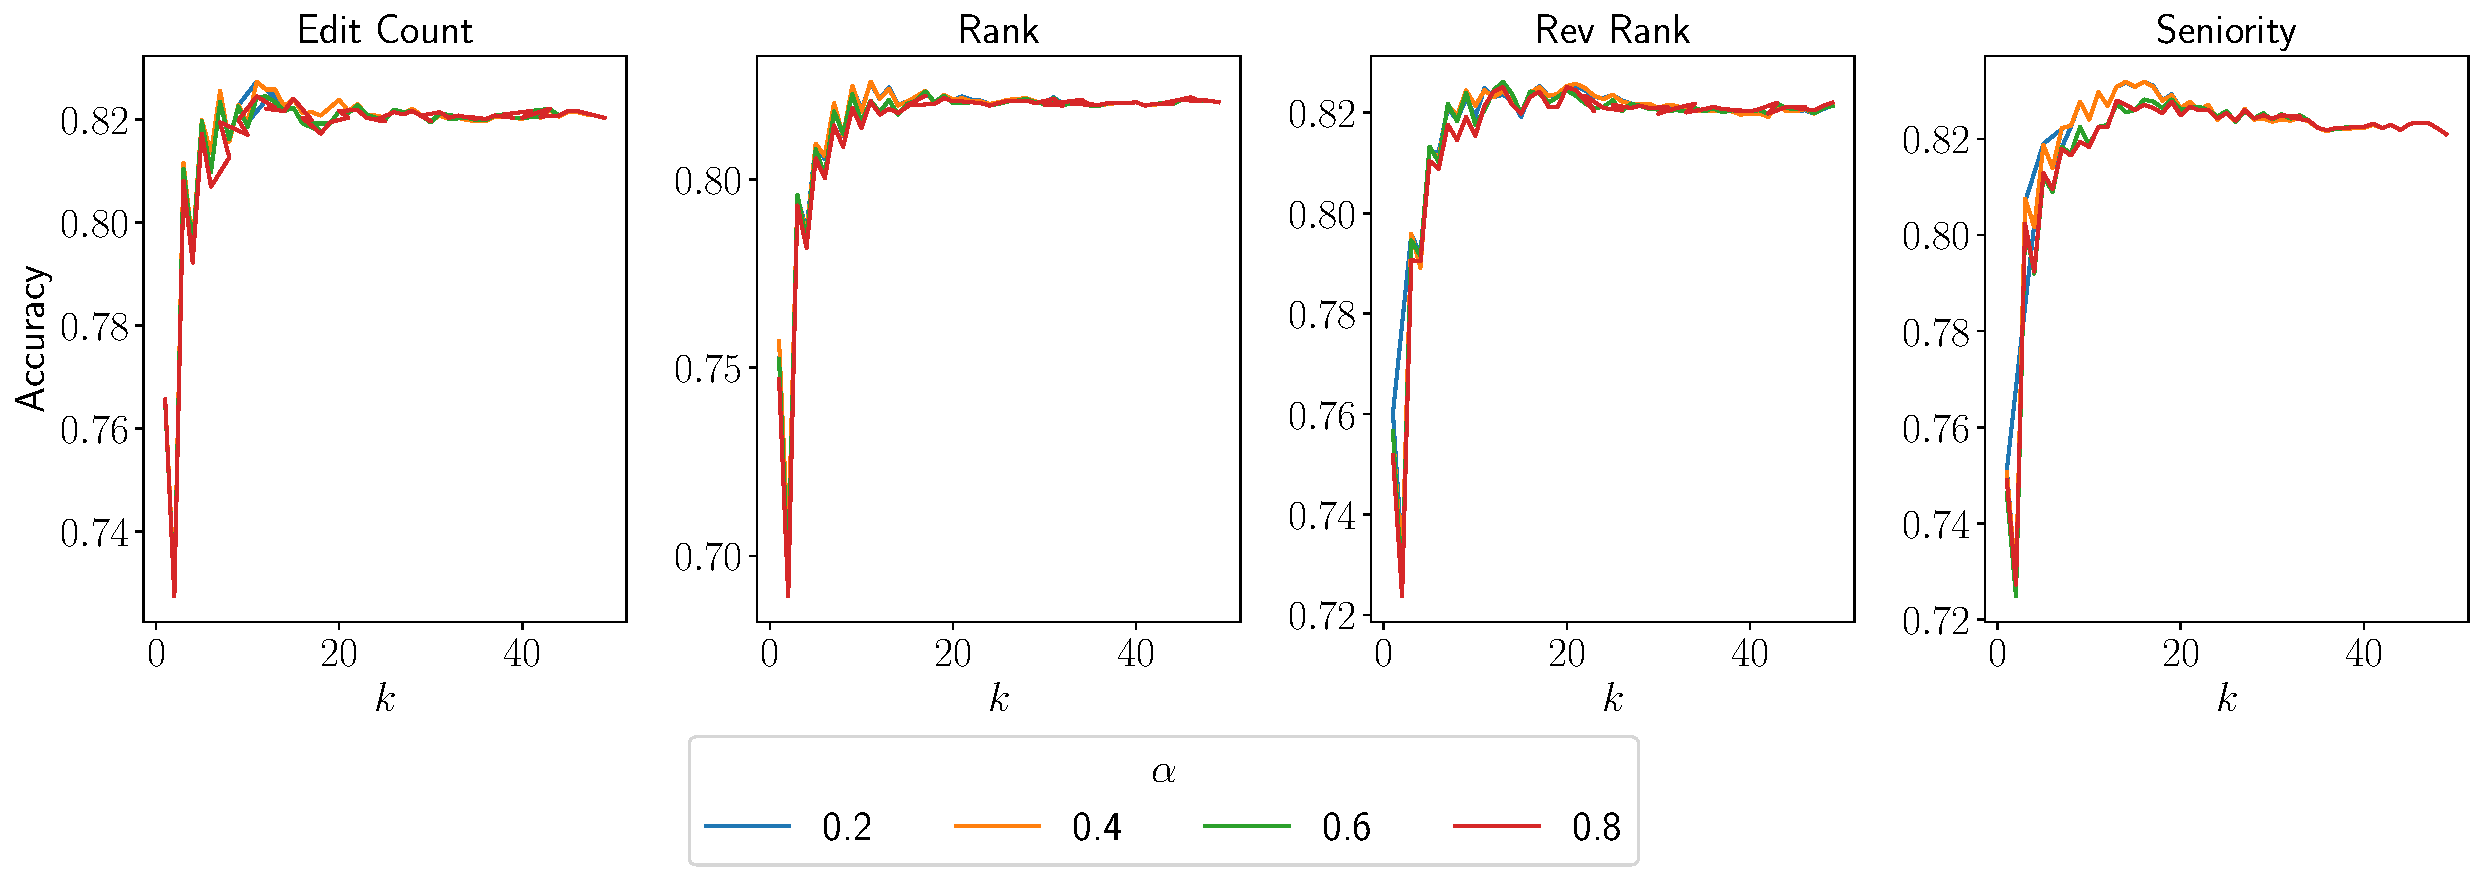
\includegraphics[width=\linewidth]{images/k_local.pdf}
    \caption{Effect of $k$ for the \localv model with different delegation rules and values of $\alpha$}
    \label{fig:local-k}
\end{figure*}
\subsection{Effect of $\alpha$}
To study the effects of the delegation parameter $\alpha$, we need to fix $k$, the delegation rule and the tally method. As the range of $k$ depends on the tally method, we split these results firstly as either using the \globalv or the \localv model.

In the \globalv model, $k \in [1,13000]$ and therefore we pick five values of $k$ and plot the accuracy of the model independently using each delegation rule. We see the results in Figure~\ref{fig:global-alpha}. There are some general trends that we can see across all the delegation rules. For small valued of $k$ the quality of predictions are low and as a result the overall accuracy is poor and usually below $50\%$. This is as expected because in the global tally scheme the top $100$ important users might not vote in all elections, therefore, the model has very few votes to tally in each election. For large values of $k$ such as $8000$, we have close to two-thirds of the unique voters and at that point the value of $\alpha$ is irrelevant as the ranking of the top $8000$ users changes very little. Moreover, almost all the votes in an election are used to calculate the tally hence the accuracy is constant close to the baseline $80\%$. For values of $k$ in the middle, we see that as $\alpha$ increases there is a gradual drop in the accuracy. This is clearly seen in the decreasing step-like pattern, for all delegation rules in Figure~\ref{fig:global-alpha}. This indicates that the \globalv model is more viscous in nature and works better for smaller values of $\alpha$.

When we consider the \localv model we see that the value of $k$ is bounded by the number of votes in a particular election. Theoretically, we can have a $k$ more than the number of votes in an election, in which case we just choose all the votes to get the tally. The average number of votes in a RfA election is $49$ and we chose the following five values $k \in \{5,10,20,40,80\}$ to analyse. We again see that for $k=5$ is accuracy is low and for $k=80$ the accuracy is close to the baseline and is stable. The reasoning is similar to the \globalv model, for small $k$ not enough votes and for large $k$ the $\alpha$ does not change ranking enough to affect the top $k$ users. The interesting trend is that unlike the \globalv model when we increase $k$ to $20$ we see that the \localv model actually performs much better than the baseline. This indicates that around the region $k=20$ there is an additional gain in performance by choosing only the important votes to tally. We also see the general trend that higher values of $\alpha$ tend to decrease the accuracy, especially for the seniority rule as seen in Figure~\ref{fig:local-alpha}. A point to note is that for most values of $k$ and delegation rules the performance drops significantly at the point $\alpha=0.5$, this indicates there might be a significant change to the ranking of voters in the \localv model at this location. Therefore votes in the local model and the global model are \textbf{more viscous than liquid}.

\subsection{Effect of $k$}
Similar to how we studied the effect of $\alpha$ above, we now take the two tally methods, delegation rules and fixed values of $\alpha \in \{0.2,0.4,0.6,0.8\}$ to understand the effect of the value of $k$. Though in an indirect way we have analysed this in the previous subsection, we now provide a more detailed view of the trends as well as the ranges to choose for $k$ when later performing the grid search. Again, we will analyse the \globalv and \localv model separately.

In Figure~\ref{fig:local-k}, we see that the \globalv model has a knee around $k=2000$, this is where we see the performance of the model approaching the baseline. It also around this region that the effect of the delegation parameter $\alpha$ is most prominent. In line with our previous analysis, we see that the smaller values of $\alpha$ perform much better than the larger values of $\alpha$ in this region. We can also verify that for both small and large $k$ the change in $\alpha$ has no effect on the accuracy of the model.

We see a similar knee for the \localv model in Figure~\ref{fig:local-k}. This time it is just before $k=20$. In this knee region, there are some differences compared to the \globalv plots. We see the effect of $\alpha$ is not as pronounced in this region. We also see that there are distinctive spikes that lead to an increase in accuracy before plateauing back to the baseline as $k$ increases. These spikes confirm the behaviour that we discussed previously in Figure~\ref{fig:local-alpha}. Around this region, the \localv model has slightly better performance than the baseline. This is again clearly evident in the $\alpha=0.4$ line for the seniority delegation rule as shown in Figure~\ref{fig:local-k}.

\subsection{Grid Search}
Gathering all the information from the previous sections on the effects of the parameter $\alpha$ and $k$, we can narrow down the search space to find the best combination of parameters. As both the \localv and \globalv models show a tendency to perform better with more viscous votes, we can restrict the search space to $\alpha \in [0.2,0.45]$. The analysis of the \globalv model shows that we need nearly $k=2500$ to get performance close to the baseline. Correspondingly for the \localv model we see for around $k=20$ we start to get much better accuracy compared to the baseline. Using these as starting points for the grid and random search of the parameter space we obtain the following best combination of model parameters as show in Table~\ref{tab:grid-search}.
\begin{table}
    \centering
    \caption{Results of the grid search of the parameters and the model accuracy}
    \label{tab:grid-search}
    \begin{tabular}{llccc}
        \toprule
        \shortstack[l]{Delegation\\ Rule} & Tally & k & $\alpha$ & Accuracy \\ \midrule
        \multirow{2}{*}{Seniority} & Global & $\approx 3500$ & $\approx 0.3$ & 0.795   \\ 
        \cmidrule{2-5}
        & Local & 15 & 0.303& 0.832  \\
        \midrule
        \multirow{2}{*}{Edit Count} & Global & $\approx 3400$ & $\approx 0.35$ & 0.791 \\
        \cmidrule{2-5}
        & Local & 15 & 0.346 & 0.826 \\
        \midrule
        \multirow{2}{*}{Rank} & Global & $\approx 3500$ & $\approx 0.43$ & 0.794\\
        \cmidrule{2-5}
        & Local & 17 & 0.289 & 0.829  \\
        \midrule
        \multirow{2}{*}{\shortstack[l]{Reveresed \\Rank}} & Global & $\approx 3200$ & $\approx 0.32$ & 0.79  \\
        \cmidrule{2-5}
        & Local & 16 & 0.298 & 0.826  \\
        \bottomrule
        \end{tabular}
\end{table}

We see that all the \localv models have performance greater than the baseline of $82\%$ with the value of $k$ close to $15$ most influential users. The value of $\alpha$ indicates that the votes in the network are sufficiently viscous in nature. 